
%--------------------------------------------------------------------
%                            Preample
%--------------------------------------------------------------------

\documentclass[aspectratio=1610,17pt,utf8]{beamer}

\usepackage[utf8]{inputenc}
\usepackage[T1]{fontenc}
\usepackage[USenglish]{babel}
\usepackage{graphicx} % graphics
\usepackage{mathabx}
\usepackage{mathpazo}
\usepackage{eulervm}


% title slide definition
\title[DS]{Distributed Systems}
\subtitle{Exam}
\author[Thomas Møller Jensen]{Thomas Møller Jensen}
\institute[Institute of Computer Science]
{
  Aalborg University\\
}

%--------------------------------------------------------------------
%                            Titlepage
%--------------------------------------------------------------------

\begin{document}

%-------------------------------------------------------------------
%                            Content
%-------------------------------------------------------------------
%                 Distributed Mutual Exclusion
%-------------------------------------------------------------------

\begin{frame}{Distributed Mutual Exclusion}
    What is a mutex? Kinda a Lock for distributed systems \ldots

    In a distributed system a mutex is for locking a shared resource in a network, traditionally in a program, a lock would be enough to handle concurrent writes/reads, but when the communication is expensive, locking the resource is harder to do.
\end{frame}

\begin{frame}{Mutex Algorithms}
    \section{Mutex algorithms}
    \begin{itemize}
        \item Centralized Algorithm
        \item Token Ring Algorithm
        \item Ricart and Agrawala's algorithm
        \item Maekawas algorithm
    \end{itemize}
\end{frame}

\begin{frame}{Centralized algortihm}
    \begin{minipage}{.45\textwidth}
        \begin{figure}
            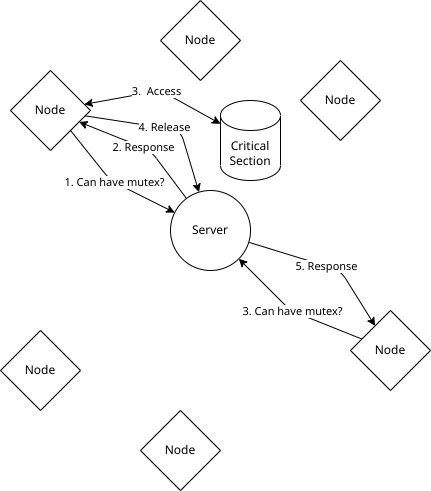
\includegraphics[width=\textwidth]{figures/1-mutex.png}
        \end{figure}
    \end{minipage}
    \begin{minipage}{.5\textwidth}
        \tiny{All three nodes highlighted are points of failure.}
    \end{minipage}
\end{frame}

\begin{frame}{Token Ring Algorithm}
    \begin{minipage}{.45\textwidth}
        \begin{figure}
            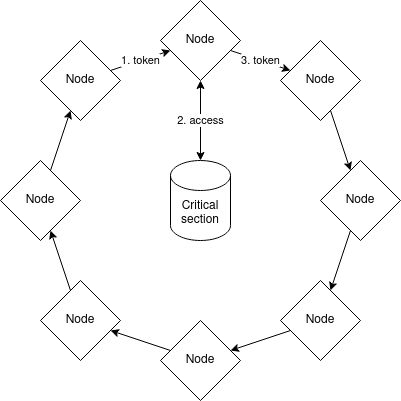
\includegraphics[width=\textwidth]{figures/1-token.png}
        \end{figure}
    \end{minipage}
    \begin{minipage}{.5\textwidth}
        \tiny{All nodes are points of failure at any given time.}
    \end{minipage}
\end{frame}

\begin{frame}{Ricart and Agrawala's algorithm}
    \begin{minipage}{.45\textwidth}
        \begin{figure}
            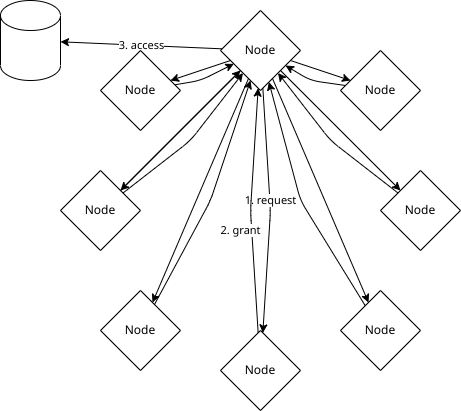
\includegraphics[width=\textwidth]{figures/1-ricart-agrawala.png}
        \end{figure}
    \end{minipage}
    \begin{minipage}{.5\textwidth}
        \tiny{All requests are multicast.\\There is a 4th step where a release is multicast to all nodes as well.\\All nodes are points of failure at any given time.}
    \end{minipage}
\end{frame}

\begin{frame}{Maekawas algorithm}
    \begin{minipage}{.45\textwidth}
        \begin{figure}
            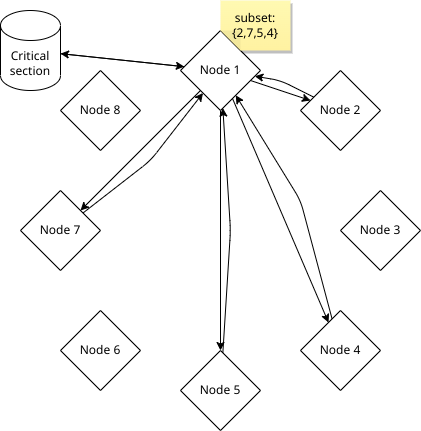
\includegraphics[width=\textwidth]{figures/1-maekawa.png}
        \end{figure}
    \end{minipage}
    \begin{minipage}{.5\textwidth}
        \tiny{Very similar to Ricart and Agrawala, but only nodes in the subset failing will result in a particular node to fail. If you're a bit smart about choosing the subsets this can be minimized.}
    \end{minipage}
\end{frame}

\begin{frame}{Performance}
    Bandwidth means Entry and Exit potential. This means how many times an acces can happen per messages.\\
    Token ring is infinite because the node itself chooses when to send the token.\\
    Ricart and Agrawala's algorithm has a bandwidth of 1+n-1 if it can do multicast in hardware, otherwise its n-1+n-1, as it will now have to unicast to everyone.
    \tiny{\begin{table}
        \begin{tabular}{|c|c|c|c|c|}
            \hline
            Algorithm & Entry & Exit & sync & Bandwidth \\\hline
            Centralized & 2 & 1 & 2 & 2 / 1 \\\hline
            Token Ring & a:n/2 w:n-1 & 1 & a:n/2 w:n-1 & $\infty$ / 1 \\\hline
            R + A & 2 & 2 & 1 & 1+n-1 or n-1+n-1 / n-1 \\\hline
            maekawa & 2 & 1 & 2 & $4 \sqrt{n}-2$ / $2 \sqrt{n}-1$ \\\hline
        \end{tabular}
    \end{table}}
\end{frame}
%-------------------------------------------------------------------
%                 Multicast/Group Communication
%-------------------------------------------------------------------

\begin{frame}{Multicast/Group Communication}
    \begin{itemize}
        \item IP Multicast
    \end{itemize}

    \begin{figure}
        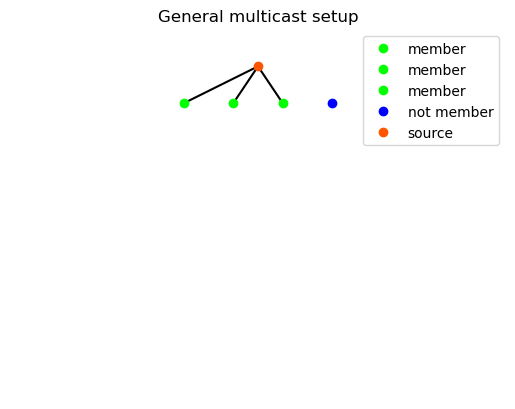
\includegraphics[width=.7\textwidth]{figures/2-multicast-group.png}
    \end{figure}
\end{frame}

\begin{frame}{IP Multicast - Hardware Support}
    Uses a protocol called IGMP

    If there's hardware support, the sender transmits one message and the intermediary devices will determine how many devices it will transmit the message to.\\
    If there is not hardware support, then the sender will have to unicast many messages at once to its receivers instead.
\end{frame}

\begin{frame}{IP Multicast - Problems}
    Out of order delivery, this can happen due to changes in routing. Consider a network with a slow and a fast intermediary node as two independant routes, if the sender sends a message through the slow node to the reciver followed by a message through the fast node, then the receiver might receive the second message before the first.
\end{frame}

\begin{frame}{Using a Sequencer}
    \begin{figure}
        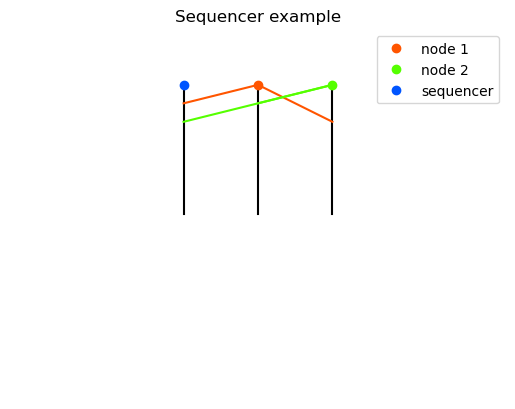
\includegraphics[width=\textwidth]{figures/2-sequencer.png}
    \end{figure}
\end{frame}

%-------------------------------------------------------------------
%                     Consensus Protocols
%-------------------------------------------------------------------

\begin{frame}{Consensus Protocols}
\end{frame}

%-------------------------------------------------------------------
%                 Replication and Consistency
%-------------------------------------------------------------------

\begin{frame}{Replication and Consistency}
\end{frame}

%-------------------------------------------------------------------
%                     Distributed Storage
%-------------------------------------------------------------------

\begin{frame}{Distributed Storage}
\end{frame}

%-------------------------------------------------------------------
%                     Big Data Analytics
%-------------------------------------------------------------------

\begin{frame}{Big Data Analytics}
\end{frame}

%-------------------------------------------------------------------
%                         Blockchains
%-------------------------------------------------------------------

\begin{frame}{Blockchains}
\end{frame}

%-------------------------------------------------------------------
%                  Peer-to-Peer Networking
%-------------------------------------------------------------------

\begin{frame}{Peer-to-Peer Networking}
\end{frame}

%-------------------------------------------------------------------
%              Internet of Things and Routing
%-------------------------------------------------------------------

\begin{frame}{Internet of Things and Routing}
\end{frame}

\end{document}